% ------------------------------------------------------------------------ %
% !TEX encoding = UTF-8 Unicode
% !TEX TS-program = pdflatex
% !TEX root = ../Tesi.tex
% !TeX spellcheck = en_US
% ------------------------------------------------------------------------ %
%
% ------------------------------------------------------------------------ %
% 	STATO DELL'ARTE
% ------------------------------------------------------------------------ %
%
\chapter{State of the Art}
%
\label{cap:statoarte}
%
% ------------------------------------------------------------------------ %
%
\section{Android OS} \label{androidos}
\par As already mentioned,in Section \ref{(motivation)} the Android operating system is an open source OS developed by Google based on Linux kernel, that can be installed on many different kind of devices.\\
In this section I want to give to the reader the basic knowledge of the Android framework to understand why and how the operating system works.
\subsection{Brief History} \label{briefhist}
\par
The Android era officially began on October 22nd, 2008, when the \textit{T-Mobile G1} launched in the United States \cite{verge2011android}.\\
At that moment the company of mountain view, Google, felt the need to create a new operating system which was able to be installed on most modern mobile phones of the time. To meet this need the Google engineers created an OS that was based on the Linux kernel, lightweight enough and ease to be used with simple hand gestures by touching the screen of the phone.\\

\begin{figure}[h]
	\centering
	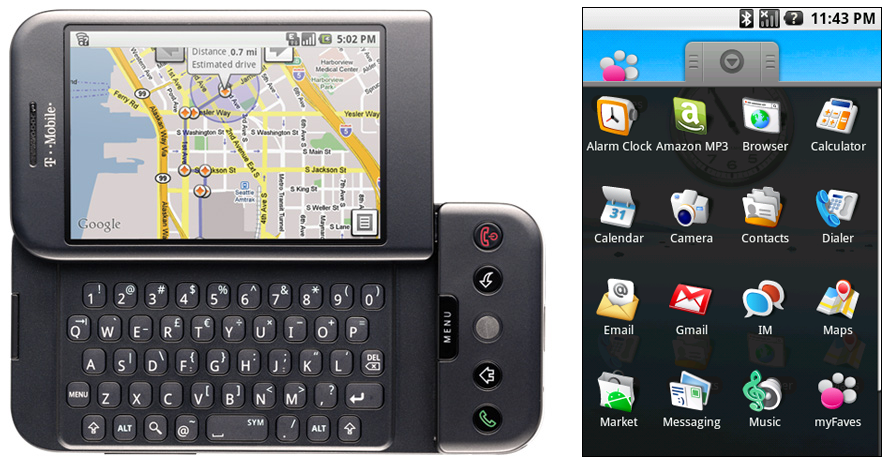
\includegraphics[width=0.8\textwidth]{T-MobileG1Android1menu}
	\caption{The T-Mobile G1 and the Android 1.0 menù}
	\label{2.1:The T-Mobile G1 and the Android 1.0 menù}
\end{figure}

The main characteristic of the OS were and are also now:
\begin{itemize}
	\item The pull-down notification window.
	\item Home screen widgets.
	\item The Android Market.
	\item Google services integration (eg. Gmail).
	\item Wireless connection technologies (eg Wi-Fi and Bluetooth)
\end{itemize}
The success of the first version of the brand new mobile operating system and the open source philosophy guaranteed the fast spread of the Android devices all over the world. In few years Google improved and released many version of the OS and with the help of the market growth Android has become a complete os. 
In the table below there is a brief description of the various distribution of the Android OS at the time of writing of this document.\\
\begin{table}[h]
	%
	\caption{Android versions}
	%
	\label{tab:vers}
	%
	\centering
	%
	\begin{tabular}{lclc}
		%
		\toprule
		%
		\textbf{Name} & \textbf{Version}  & \textbf{Release Date} & \textbf{API Level}\\
		%
		\midrule
		%
		Alpha &	1.0 & September 23, 2008 & 1 \\
		Beta & 1.1 & February 9, 2009 & 2 \\
		Cupcake & 1.5 & April 27, 2009 & 3 \\
		Donut &	1.6 & September 15, 2009 & 4 \\
		Eclair & 2.0 – 2.1 & October 26, 2009 & 5–7 \\
		Froyo & 2.2 – 2.2.3 & May 20, 2010 & 8 \\
		Gingerbread & 2.3 – 2.3.7 & December 6, 2010 & 9–10 \\	
		Honeycomb & 3.0 – 3.2.6 & February 22, 2011 & 11–13 \\
		Ice Cream Sandwich & 4.0 – 4.0.4 & October 18, 2011 & 14–15 \\
		Jelly Bean & 4.1 – 4.3.1 & July 9, 2012 & 16–18 \\
		KitKat & 4.4 – 4.4.4 & October 31, 2013 & 19 \\
		Lollipop & 5.0 – 5.1.1 & November 12, 2014 & 21–22 \\
		Marshmallow & 6.0 – 6.0.1 & October 5, 2015 & 23 \\
		Nougat & 7.0 – 7.1.1 & August 22, 2016 & 24–25 \\
		%
		\bottomrule
		%
	\end{tabular}
	%
\end{table}
 As we can see in \tablename~\ref{tab:vers} there are, currently, 25 level of the Android \textit{API} (Application programming interface
 ) which developers can use to build Android applications. In particular various API levels introduce innovations in the OS but, applications developed using an higher \textit{API level} can not be executed in a device running lower versions of the operating system. This is a second major limitations for the \textit{"Android ecosystem"}, moreover as mentioned before, the Android OS is released under an open source license, which is great for the developer, but which prevents Google to provide updates, in a centralized way, to all devices. For this reason there are currently many active devices running different versions of the mobile OS, as we can check in \tablename~\ref{tab:chart}, which shows, in percentage, the fragmentations of active machines running Android OS.\\
 \begin{table}[h]
 	%
 	\caption{Android OS versions fragmentation}
 	%
 	\label{tab:chart}
 	%
 	
 	%
 	\begin{minipage}{0.5\textwidth}
 		\centering
 		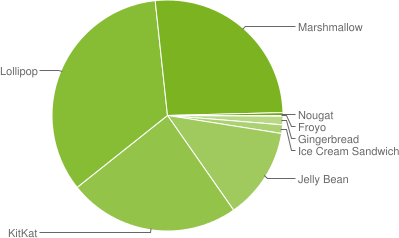
\includegraphics[width=0.9\textwidth]{androidversionchart}
 		 \captionof{figure}{Android OS fragmentation chart}
 		\label{2.2:Android fragmentation chart}
 		
 	\end{minipage}
 ~\hfill~
 \begin{minipage}{0.5 \textwidth}
 	\centering
 	\begin{tabular}{ccc}
 		%
 		\toprule
 		%
 		\textbf{Version}  & \textbf{API Level} & \textbf{Distribution}\\
 		%
 		\midrule
 		%
 		2.2 & 8 & 0.1\% \\
 		2.3.3 - 2.3.7 & 10 & 1.2\% \\
 		4.0.3 - 4.0.4 & 15 & 1.2\% \\
 		4.1.x & 16 & 4.5\% \\
 		4.2.x & 17 & 6.4\% \\
 		4.3 & 18 & 1.9\% \\
 		4.4 & 19 & 24.0\% \\
 		5.0 & 21 & 10.8\% \\
 		5.1 & 22 & 23.2\% \\
 		6.0 & 23 & 26.3\% \\
 		7.0 & 24 & 0.4\% \\
 		%
 		\bottomrule
 		%
 	\end{tabular}
\end{minipage}
 	%
 \end{table}
Data in \tablename~\ref{tab:chart} were collected during a 7-day period ending on December 5, 2016, by Google. Any versions with less than 0.1\% distribution are not shown \cite{devandroiddash}.
\subsection{Structure}
\par
Android is an operating system based on the Linux kernel. The project responsible for developing the Android system is called the \textit{Android Open Source Project (AOSP)} and it lead by Google.
\begin{figure}[h]
	\centering
	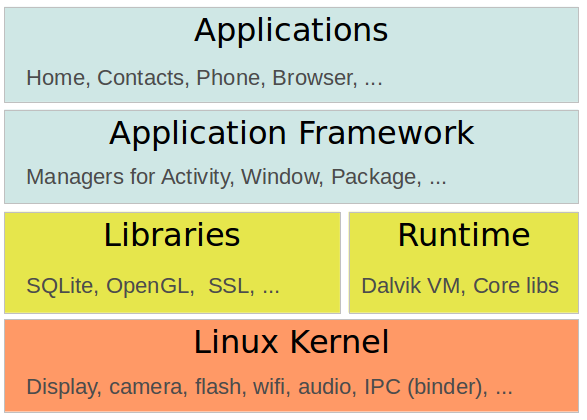
\includegraphics[width=0.8\textwidth]{oslevels}
	\caption{Android OS 4 layers}
	\label{fig:2.3}
\end{figure}

The OS can be divided into the four layers as depicted the \figurename~\ref{fig:2.3}. An Android application developer typically works with the two layers on top to create new Android applications \cite{vogel2016android}.

\subsubsection{Linux Kernel} 
The Linux Kernel is the most flexible operating system that has ever been created. It can be tuned for a wide range of different systems, running on everything from a radio-controlled model helicopter, to a cell phone, to the majority of the largest supercomputers in the world \cite{hartman2006linux}. This is in practice the communication layer for the underlying hardware.
\subsubsection{Runtime and Libraries}
Runtime is the term used in computer science to designate the software that provides the services necessary for the execution of a program.There are two different \textit{"runtime systems"} which can work with the Android OS:
\begin{itemize}
	\item \textit{Dalvik VM} is an optimized version for low memory devices of the \textit{Java Virtual Machine (JVM)} used in Android 4.4 and earlier version. It is stack based and it works by converting using a \textit{just-in-time (JIT)}, each time an application is executed, Android's \textit{bytecode} into machine code.
	\item \textit{ART (Android Runtime)} introduced with Android 4.4 KitKat. This runtime uses an \textit{AOT (Ahead-of-Time)} approach, with which code is compiled during the installation of an application and then is ready to be executed.
\end{itemize}
\par Standard Android libraries are for many common framework functions, like, graphic rendering, data storage, web browsing. \cite{vogel2016android}. This layer contains also standard \textit{java libraries}.
\subsubsection{Application Framework}\label{appframework}
The application framework is the layer that contains the Android components for the application such as activities, fragments, services and so on. 
\subsubsection{Applications}
Applications are pieces of software written in \textit{java code} running on top the other layers.

\subsection{Application Framework}
In this section I want to give some details of the application composition and work flow to better understand the subsequent sections in which I will describe the given problem and the proposed solution.\\
As briefly described in Section \ref{appframework}, the Android application framework \textit{("AppFramework")} is the core of the Android \textit{development API}. It contains useful and needed components to build native apps.\\
The main components with which each application is composed are:

\subsubsection{Intents}\label{intents} Intents are objects that initiate actions from other app components, either within the same program \textit{(explicit intents)} or through another piece of software on the device \textit{(implicit intents)}.
Acconrding to the official Google's Android for developer documentation, an Intent is a sort of messaging object which can be used to request an action from another application component (eg. activities). There are three fundamental use cases:
\begin{itemize}
	\item Starting an activity: we will see that activities represents a single screen in Android applications, intents allow to start activities by describing them and carrying any necessary data.
	\item Starting a service: I will explain later in deeper details that services are component which performs operations in background. As for the activities, services are initialized through intent and in the same way they describe the service to start and carries any necessary data.
	\item Delivering a broadcast: broadcast is a message that any app can receive. The system delivers various broadcasts for system events, such as when the system boots up or the device starts charging.
\end{itemize}

As already mentioned there are mainly two categories of intents:
\begin{itemize}
	\item explicit intents, used when it is needed to start component within the same application. As the name implies explicit intents call components by using by name (the full \textit{class object} name), for example, it is possible to start a new activity in response to a user action or start a service to download a file in the background.
	\item implicit intents do not name a specific component, but instead declare a general action to perform, which allows a component from another app to handle it. For example, if you want to show the user a location on a map, you can use an implicit intent to request that another capable app show a specified location on a map \cite{devandroidintent}.
\end{itemize}

\begin{figure}[h]
	\centering
	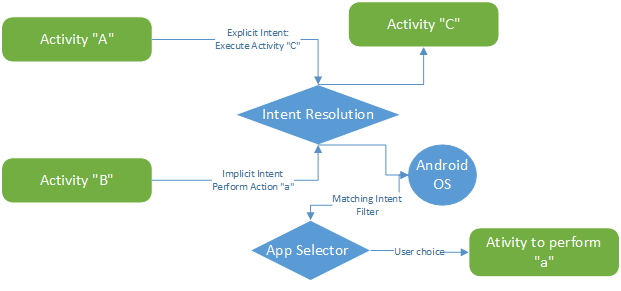
\includegraphics[width=0.9\textwidth]{intentresolution}
	\caption{Intent resolution mechanism}
	\label{fig:2.4}
\end{figure}

The \figurename~\ref{fig:2.4} explains well how an intent is resolved by the OS whether it is implicit or explicit. When an implicit intent needs to be resolved, the OS searches applications which can handle it by means of \textit{intent filters}.A Intent filter specifies the types of intents that an activity, service, or broadcast receiver can respond to. The Android System searches all apps for an intent filter that matches the intent to be resolved. When a match is found, the system starts the matching component, or, if there are more than one, let the user select the preferred action to be performed.

\subsubsection{Activities} Activities are one of the fundamental building blocks of apps on the Android platform. They serve as the entry point for a user's interaction with an app, and are also central to how a user navigates within an app. \cite{devandroidactivity}. An activity is the entry point for interacting with the user. It represents a single screen with a user interface \textit{GUI}: in this way activities are containers for other Android's GUI elements (eg. buttons, textviews,...).

\subsubsection{Services} A service is a general-purpose entry point for keeping an app running in the background for all kinds of reasons. It is a component that runs in the background to perform long-running operations or to perform work for remote processes. A service does not provide a user interface \cite{devandroifundamentals}. 

\subsubsection{Broadcast Receivers} Broadcast Receivers are components that enable the system to deliver events to the app outside of a regular user flow, allowing the app to respond to system-wide broadcast announcements. Because broadcast receivers are another well-defined entry into the app, the system can deliver broadcasts even to applications that aren't currently running \cite{devandroifundamentals}.

\subsection{Security}\label{androidsecurity}
\par
As described in Section \ref{briefhist}, Android was born to be a good mobile OS and it is mainly for this reason that the system is designed to protect personal and sensible data form malicious guys.\\
Like the rest of the system, Android's security model also takes advantages of the security features offered by the Linux kernel. Linux is a \textit{multiuser OS} and its kernel can isolate user data from one another: one user can not access another user's file unless explicitly granted permission. Android takes advantages of this user isolation, considering each application a different user provided with a dedicated \textit{UID (User ID)} \cite{elenkov2014android} Android in fact, is designed for smartphones that are personal devices and do not need, usually, a multi physical user support.
The most important security techniques adopted by Android are:

	\subsubsection{Application Sandboxing} Android automatically assigns a unique \textit{AppID} (Linux UID) when an application is installed and then executed that specific app in a dedicated process as that UID. This technique isolate all the applications at process level and additionally each app has permissions to read/write a specific and dedicated directory.
	
	\subsubsection{Permissions} Since application are sandboxed and do not have the rights to read/write date outside them, it is possible to grant additional rights to android applications by explicitly asking them. Those access rights are called \textit{permission}. Applications can request permissions by listing them in a configuration file called \textit{android manifest}. In Android 5.1 and earlier versions permission are inspected and granted at installation time, when the user is alerted with a dialog box in which are listed permissions the application to be installed needs to work properly and when granted cannot be revoked. Starting from android 6.0 permission are asked the first time that an application need them, and when are granted they can be revoked manually in the OS settings for that specific application.
	
		\begin{figure}[h]
		\centering
		\begin{minipage}[c]{.45\textwidth}
			\centering\setlength{\captionmargin}{0pt}%
			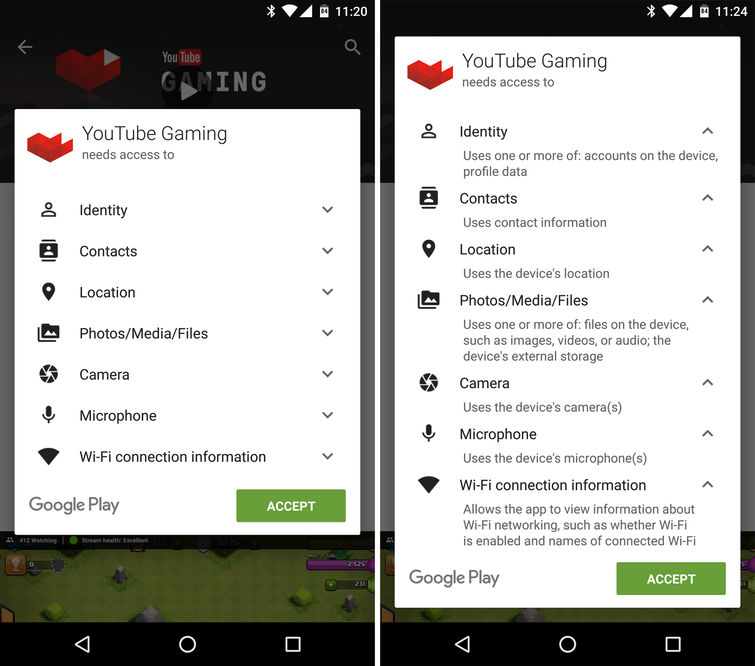
\includegraphics[width=.9\textwidth]{51permissions}
			\caption{Android 5.1- permission example}
		\end{minipage}%
		\hspace{10mm}%
		\begin{minipage}[c]{.45\textwidth}
			\centering\setlength{\captionmargin}{0pt}%
			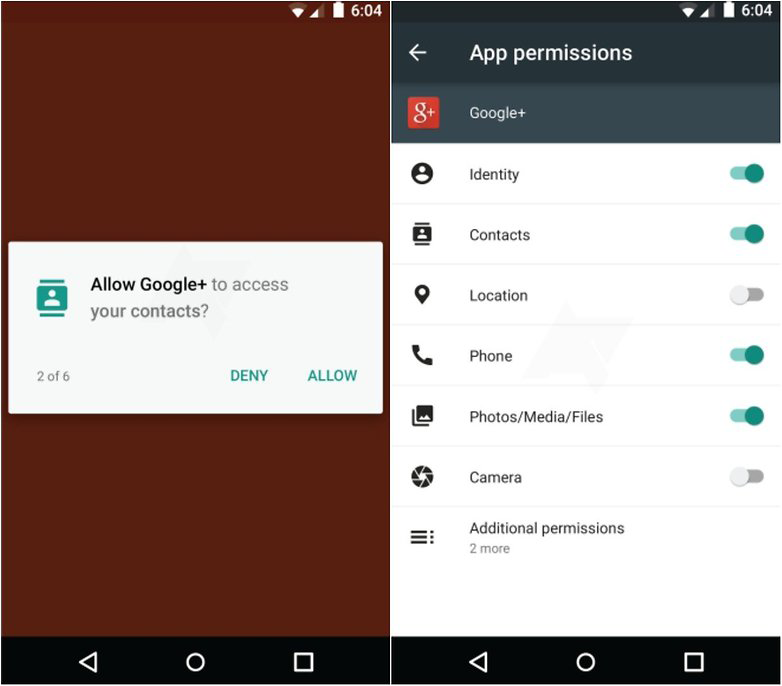
\includegraphics[width=.9\textwidth]{60permissions}
			\caption{Android 6.0+ permission example}
		\end{minipage}
		\caption{Android permission Examples\label{fig:Andorid permission Examples}}
	\end{figure}

	\subsubsection{SeLinux} Security Enhanced Linux, is a \textit{mandatory access control (MAC)} system for the Linux operating system. With a MAC the operating system constrains the ability of a subject or initiator to access or generally perform some sort of operation on an object or target. Starting in Android 4.3, SELinux provides a mandatory access control (MAC) umbrella over traditional discretionary \textit{access control (DAC)} environments. For instance, software must typically run as the root user account to write to raw block devices. In a traditional DAC-based Linux environment, if the root user becomes compromised that user can write to every raw block device. However, SELinux can be used to label these devices so the process assigned the root privilege can write to only those specified in the associated policy.
 	In this way, the process cannot overwrite data and system settings outside of the specific raw block device \cite{secure2017android}.

\subsection{Connectivity}\label{connectivity}
\par
As already explained previously many Android design choices are due to the fact that it was thought for mobile devices which must have connectivity to intercommunicate among them.\\
With the evolution of various wireless communication technologies, Android devices, nowadays, are equipped whit different kinds of modulus, the most common are:
\begin{itemize}
	\item Wi-Fi
	\item Bluetooth
	\item NFC
	\item Cellular Network
\end{itemize}
The Android Os provide a full library to operate with these technologies and it is possible to integrate in applications the possibility to communicate over these wireless modules.
With the \textit{Android connectivity API} data can be send and received in an efficient way.\\\\
\par
I have only quickly listed some features and possible issues of my source, to have a complete idea it is possible to read all the official Android documentation in \cite{devandroifundamentals}.
 
\section{Distributed System} \label{distsys}
In this section I want to give to the reader some basics about distributed systems, including technical details and examples to make the proposed solution easier to understand.
\subsection{Definition}\label{distdef}
\textit{A distributed system is a collection of independent computers that appears to its users as a single coherent system.}\\
This definition has several important aspects. The first one is that a distributed system consists of components (i.e., computers) that are autonomous. A second aspect is that users (be they people or programs) think they are dealing with a single
system. This means that one way or the other the autonomous components need to collaborate \cite{tanenbaum2010distributed}.\\
\begin{figure}[h]
	\centering
	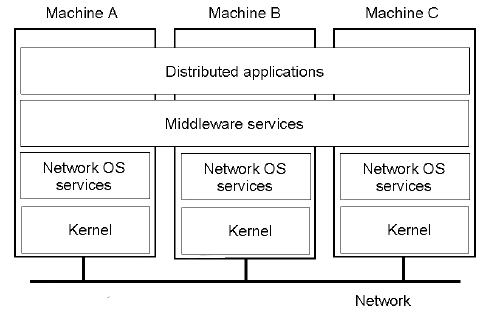
\includegraphics[width=0.8\textwidth]{distributedsystem}
	\caption{Distributed system structure}
	\label{fig:2.8}
\end{figure}
In \figurename~\ref{fig:2.8} it is possible to see how can be structured a distributed system: a the top we have the real distributed application, which is the final interface to be used, under which it is possible to have different combinations of services used to make communicate different machines that may use different operating systems. The real magic is done by the layer called \textit{middleware service} in the picture. A middleware in computer science is a set of software which act as intermediaries between structures and computer programs, allowing them to communicate in spite of the diversity of protocols or running OSs.

\subsection{Challenges} \label{chall}
There are many challenges in distributed systems field: distributed applications are often really complex and easily exposed to physical and technical failures because of their nature. Major challenges and property to be considered when developing a system of this kind are:

\begin{figure}[h]
	\centering
	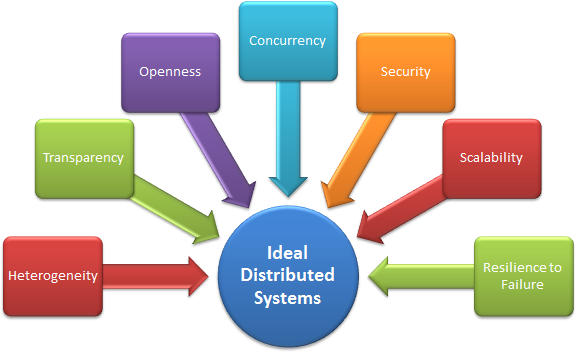
\includegraphics[width=0.8\textwidth]{challengesdistributedsystems}
	\caption{Distributed system challenges}
	\label{fig:2.9}
\end{figure} 

\begin{itemize}
	\item Heterogeneity, is a major challenge because there are many different component to be considered, distributed systems may be developed for example for different hardware, networks, operating systems and programming languages.
	\item Openness, determines whether a system can be extended and reimplemented in various ways, so distributed systems should use standards as much as possible. Developers should always choose the simplest ways during design and implementation phases.
	\item Security, is crucial in many areas of computer science and specially in distributed systems, where data are exchanged by a several number of machines.
	\item Scalability, is the ability to easily increase the size of the system in terms of users/resources and geographic
	span.
	\item Failure handling, is important because having different components working together to a common goal means that distributed system can fail in many ways. This raises some issue: it would be nice id distributed systems can detect, mask and tolerate failures.
	\item Concurrency in distributed systems is a matter of
	fact, access to shared resources (information or services)
	must be carefully synchronized.
	\item Transparency level are listed in \tablename~\ref{tab:transparency}
\end{itemize}

	\begin{table}[h]
		%
		\caption{Transparency levels}
		%
		\label{tab:transparency}
		%
		\centering
		%
		\begin{tabular}{lp{0.75\textwidth}}
			%
			\toprule
			%
			\textbf{Transparency} & \textbf{Description}\\
			%
			\midrule
	%
			Access & Hide differences in data representation and how a resource is accessed\\
			Location & Hide where a resource is located\\
			Migration & Hide that a resource may move to another location\\
			Relocation & Hide that a resource may be moved to another location while in use\\
			Replication & Hide that a resource may be shared by several competitive users\\
			Concurrency & Hide that a resource may be shared by several competitive users\\
			Failure & Hide the failure and recovery of a resource\\
			Persistence & Hide whether a (software) resource is in memory or on disk\\
			%
			\bottomrule
			%
		\end{tabular}
		%
	\end{table}

\subsection{Comunication Model} \label{mpi}
\par
There are, in distributed system literature, some well known techniques to let communicate machines, programs and components. Each of the methods described later exploits the network protocols by acting as a middleware: they use and mask lower layer protocols to provide ready to use communication services.

\subsubsection{Remote procedure call (RPC)} RPC is a paradigm in which a client process invokes a remotely located procedure (a server process), the remote procedure executes and sends the response back to the client \cite{Jerome2009Principles}.
\begin{figure}[h]
	\centering
	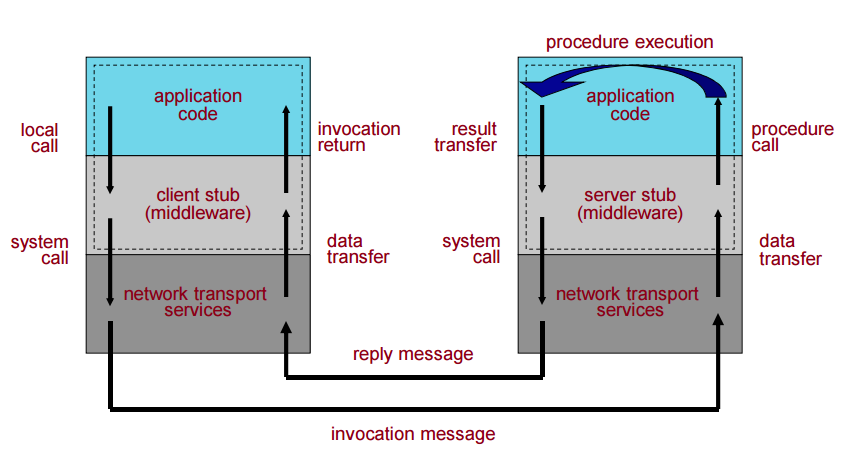
\includegraphics[width=0.8\textwidth]{rpc}
	\caption{RPC in detail}
	\label{fig:2.10}
\end{figure} 
As described in \figurename~\ref{fig:2.10} RPC provides the localization of the code to be executed exploiting the network transport services, create a message which can be serialized and transferred over a standard network protocol and then provides methods to de-serialize the message and convert in into a standard local procedure call in the receiver machine. Very important in this mechanism is the concept of \textit{ILD} (Interface definition language) which raises the level of abstraction of the service by separating the interface from its implementation: in this way RPC can be language independent by generating automatic translations from IDL to target language.  
\subsubsection{Remote method invocation (RMI)} \label{RMI} RMI exploits the same idea of RPC but with different programming constructs: it is designed to let communicate object oriented (OO) programming languages.
\begin{figure}[h]
	\centering
	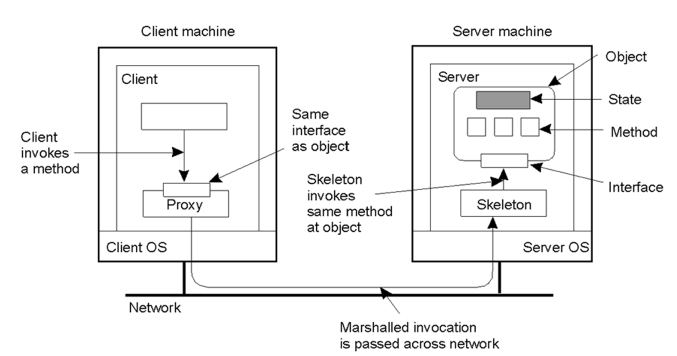
\includegraphics[width=0.8\textwidth]{rmi}
	\caption{RMI in detail}
	\label{fig:2.11}
\end{figure} 
The \figurename~\ref{fig:2.11} shows in detail how RMI is supposed to work. Like RPC, RMI uses an IDL which is designed to support OO programming languages features such as inheritance and exception handling.
\subsubsection{Message oriented} \label{messageo} Message oriented communication is a style based and centered on the notion of simple messages and events.The most straightforward example of it is \textit{message passing}. Typically message passing is implemented directly on the network sublayers (eg. sockets). Message passing differs from conventional programming where a process, subroutine, or function is directly invoked by name. 
\begin{table}[h]
	%
	\caption{Comparison between communication models}
	%
	\label{tab:comp}
	%
	\centering
	%
	\begin{tabular}{p{0.45\textwidth}p{0.45\textwidth}}
		%
		\toprule
		%
		\textbf{RPC/RMI} & \textbf{Message Oriented} \\
		%
		\midrule
		%
		& \\
	      \begin{minipage}[t]{0.45\textwidth}
	     	\begin{itemize}
	     		\item natural programming abstractions
	     		\item point to point communication
	     		\item designed for synchronous communication
	     		\item high coupling between the caller and the callee
	     	\end{itemize}
	     \end{minipage} &  \begin{minipage}[t]{0.45\textwidth}
	     \begin{itemize}
	     	\item centered around the notion of message/event
	     	\item multipoint support
	     	\item usually asynchronous
	     	\item high level of decoupling
	     \end{itemize}
     \end{minipage} \\
  & \\
		
		%
		\bottomrule
		%
	\end{tabular}
	%
\end{table}
In \tablename~\ref{tab:comp} are shown the most significant differences between RPC/RMI approach and message communication models. Moreover there are some implementation of message passing at middleware layer like \textit{publish-subscribe} which is further explained in the following paragraph.

\subsection{Architectures}
\par
There are actually many different kinds of distributed systems which can be classified by means of their architecture composition.
\subsubsection{Client-Server}
\begin{figure}[h]
	\centering
	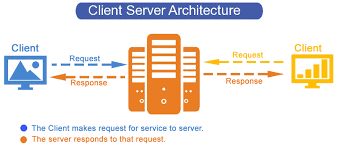
\includegraphics[width=0.8\textwidth]{clientserver}
	\caption{Client server architecture}
	\label{fig:2.12}
\end{figure} 
 Client-Server is the most common architecture in computer systems, there are many variants depending on the internal division of its components but it has a common separation of duties. Server side components are passive and wait for clients invocations.Client computers provide an interface to allow a computer user to request services of the server and to display the results it returns. Servers wait for requests to arrive from clients and then respond to them. Ideally, a server provides a standardized transparent interface to clients so that clients need not be aware of the specifics of the system (i.e., the hardware and software) that is providing the service. The communication adopted by these kind of systems is message oriented or through RPC.


\subsubsection{Peer-to-Peer (P2P)}\label{P2P}
\begin{figure}[h]
	\centering
	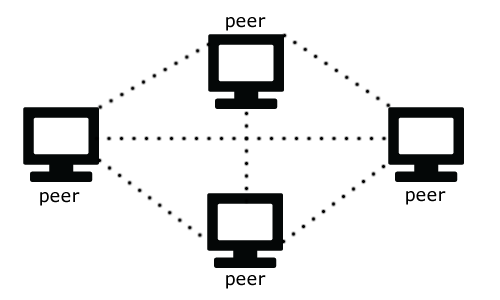
\includegraphics[width=0.8\textwidth]{p2p}
	\caption{P2P architecture}
	\label{fig:2.13}
\end{figure} P2P is a fully distributed architecture which in contrast to client-server has not a centralized service provider. Peers are both clients and servers themselves, P2P promotes sharing of resources and services trough direct exchange between peers. Compared to a centralized client-server architecture a P2P net scales better and typically does not have a single point of failure. 

\subsubsection{REST style} Representational State Transfer (REST) is a style of architecture based on a set of principles that describe how networked resources are defined and addressed.An application or architecture considered RESTful or REST-style is characterized by:
\begin{itemize}
	\item state and functionality are divided into distributed resources,
	\item every resource is uniquely addressable using a uniform and minimal set of commands (typically using HTTP commands of GET, POST, PUT, or DELETE over the Internet),
	\item the protocol is client/server, stateless, layered, and supports caching.
\end{itemize}



\subsubsection{Event based} Event based is an architecture in which components collaborate by exchanging information about occurring events. In particular components in the net can \textit{publish} notifications about the events they observe or \textins{subscribe} to events they are interested to be notified about. This architecture can be fully distributed with all the same nodes or can have some semi-centralized nodes which are specialized in computing events or routing messages. Communication is, in this case, purely message based asynchronous and multicast. 
\begin{figure}[h]
	\centering
	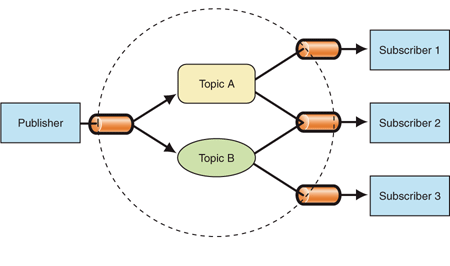
\includegraphics[width=0.8\textwidth]{publishsubscribe}
	\caption{Publish-subscribe architecture}
	\label{fig:2.14}
\end{figure} \\\\\\

\subsection{Naming}
%descrivere problemi di naming e 0 conf
Naming is one of the major issues when building distributed systems, in fact, it is often impossible to know a priori, exactly the addresses and port services of all the components in a distributed network, especially when the system allows dynamic connections and disconnections. It is important therefore, to adopt a naming model or service, to automatize components discovery and connections, when running a distributed system. To understand how naming models e solvers work it is important to introduce some naming concepts in the distributed systems paradigm.\\
In distributed systems names are used to identify a wide variety of resources such as computers, hosts, files, services as well as users. Names are usually accessed by an \textit{access point} which is a special entity characterized by an \textit{address}. Addresses are just special names which can be used by communications protocol to connect different machines. For this reason it is important to know access point addresses because otherwise it would be impossible to connect components. Dynamic systems let components change access points frequently, so having \textit{location-independent} names is much more convenient than known static addresses which can change during system execution. \textit{Identifiers} such that they never change during the lifetime of an entity, are unique, and can not be exchanged between different entities. In this way, using identifiers, it is possible to split the naming problem in two: mapping a name to the entity and then locating the entity itself.
Naming schemes are the solution to the first problem, and the most used ones are:
\begin{itemize}
	\item \textit{Flat naming}, or unstructured, are simple identifiers represented by random strings of bits.An important property of such a name is that it does not contain any information whatsoever on how to locate the	access point of its associated entity \cite{tanenbaum2010distributed}.
	\item \textit{Structured naming} are composed from simple, human-readable names, not only file naming,but also host naming on the Internet follow this approach,in fact, flat names are good for machines, but are generally not very convenient for humans to use \cite{tanenbaum2010distributed}.
	\item \textit{Attribute based naming} is a way to describe an entity in terms of \textit{(attribute, value)}
	pairs. Flat and structured names generally provide a unique and location-independent
	way of referring to entities. Moreover, structured names have been partly
	designed to provide a human-friendly way to name entities so that they can be
	conveniently accessed. In most cases, it is assumed that the name refers to only a
	single entity. However, location independence and human friendliness are not the
	only criterion for naming entities \cite{tanenbaum2010distributed}. Using attribute based naming is possible to give more information about entities or services to be found.
\end{itemize}
The solution to the second problem is called \textit{name resolution}. Name resolution in the process of obtaining the address of a valid access point of an entity having its name. Name resolution services highly depends of the naming model adopted by a system.\\
For sake of brevity here are not reported any detail of name resolution systems, but only basic naming notions to understand author's design choices in solving the thesis problem. 


\section{Technical Background}\label{techback}
This section has the aim to give to readers a useful technical background to understand the implemented and proposed solution in the following chapters.
\subsection{Liquid Computing}\label{liquid computing}
The term was coined for Apple's liquid computing feature and refers to a style of work-flow interaction of applications and computing services across multiple devices, such as computers, smartphones, and tablets.\\
In a liquid computing approach, a person might work on a task on one device, then go to another device that detects the task in progress at the first device and offer to take over that task.
In other terms liquid computation is a sort of what is called \textit{ubiquitous computing} which is a model of man-machine interaction in which information elaboration is integrated in everyday objects.
\subsubsection{Examples}
There are some implementation of this concept in mobile computer science, the most significant are:
\begin{itemize}
	\item Apple continuity, is a system, developed by Apple, with which a user can initiate a task on one device and end the task on another. For example it is possible to answer a call with a computer without using the phone.
	\item Google chrome and Gmail, developed by Google, allow users to surf the web and to write email on every available device as if they were using a single device. By registering a Google account chrome can save the navigation history of the user and show it on any logged device. In the same way Gmail saves automatically emails and for example is possible to start writing an email on a desktop pc and then completing and sending that email on a smartphone.
	\item Microsoft One Drive sync is a system, developed by microsoft to allow users to synchronize file and settings among their devices like desktops, notebooks smartphones and so on.
\end{itemize}

\subsection{Java network programming}
Since the entire Android development API is written in Java, the whole implemented solution will be in Java.\\ Java is a known general-purpose computer programming language that is concurrent, class-based, object-oriented \cite{gosling2005the}, and specifically designed to have as few implementation dependencies as possible. It is intended to let application developers "write once, run anywhere" (WORA) \cite{computer2002write}, meaning that compiled Java can run on all platforms that support Java without the need for recompilation.\\
The \textit{Java Development Kit (JDK)} includes many utility libraries, useful to develop any kind of application, I want to focus attention on network programming libraries to be used when developing distributed system using Java.
There are, currently many different possibilities among which to choose to let Java software components communicate on the network, the most simple and common are \textit{Sockets} and \textit{Java RMI}.
\subsubsection{Sockets} \label{socket} Sockets are abstractions through which an application may send and receive data, in much the same way as an open file handle allows an application to read and write data to stable storage.
A socket allows an application to plug in to the network and communicate with other applications that are plugged in to the same network. Information written to the socket by
an application on one machine can be read by an application on a different machine and vice versa \cite{calvert2011tcp}.
Different types of sockets correspond to different underlying protocol suites and different
stacks of protocols within a suite.
\begin{figure}[h]
	\centering
	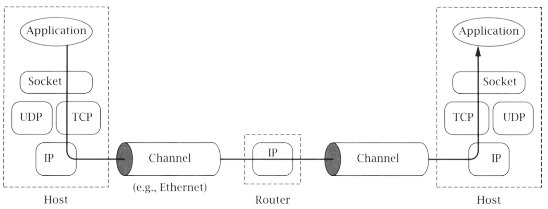
\includegraphics[width=0.9\textwidth]{tcpip}
	\caption{TCP/IP sockets}
	\label{fig:2.15}
\end{figure}
In \figurename~\ref{fig:2.15} it is shown the working mechanism of a \textit{TCP/IP socket}: the application exploiting the socket communicate using the TCP transport layer and the IP networking layer. In this way it is possible to read/write packets knowing four variables: socket TCP port number and IP address for the sender and the receiver.\\
Java provide a network library with which is very easy to implement a client/server simple application using TCP/IP sockets. 
%The following snippet of code are provided to give a concrete Java client/server application using sockets.
%modo per inserire codice java da file
%\lstinputlisting[language=Java , caption=DateServer example]{Codici/DateServer.java}
%\lstinputlisting[language=Java , caption=DateClient example]{Codici/DateClient.java}
%Comments in the example gives the full explanation of how simple client/server Java application using TCP sockets works.

\subsubsection{Java RMI} Java RMI it is an implementation of \textit{Remote Method Invocation} previously discussed in Section \ref{RMI}. It represent the best alternative to sockets when building network applications. Java RMI is a complete middleware itself, in fact, it raises the level of abstraction of the network communication environment.
\begin{figure}[h]
	\centering
	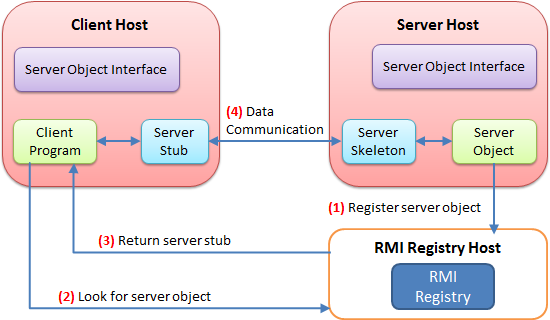
\includegraphics[width=0.9\textwidth]{JavaRMI}
	\caption{Java RMI structure}
	\label{fig:2.16}
\end{figure}

Remote method invocation allows applications to call object methods located remotely, sharing resources and processing load across systems. Unlike other systems for remote execution which require that only simple data types or defined structures be passed to and from methods, RMI allows any Java object type to be used - even if the client or server has never encountered it before. RMI allows both client and server to dynamically load new object types as required.
\subsection{Zeroconf}\label{zeroconf} Zero-configuration networking or \textit{Zerconf} is a set of technologies that automatically creates a usable computer network based on the TCP/IP Internet paradigm, when computers or network peripherals are interconnected. \\
The aim of this technology is to let users easily connects to various local network services, without the need of configurations. The architecture of Zeroconf is built around simplicity. It should be as easy for an end users to connect a printer or locate streamed music as it is for him to turn on light bulb \cite{cheshire2006zero}.\\
It is built on three core technologies: automatic assignment of numeric network addresses for networked devices, automatic distribution and resolution of computer hostnames, and automatic location of network services.\\

\subsubsection{Service Discovery and Name Resolution}
To the end user, the most important facet of Zeroconf is the ability to easily browse for available services in the network. With Zeroconf you browse for services, not for hardware \cite{cheshire2006zero}. Internet protocols use IP addresses for communications, but these are not really human-readable; IPv6 in particular uses very long strings of digits that are not easily entered manually. To address this issue, the internet has long used the Domain Name System (DNS), which allows human-readable names to be associated with IP addresses, and includes code for looking up these names from a hierarchical database system. Users type in common names, like wikipedia.org, which the computer's DNS software looks up in the remote DNS databases, translates to the proper IP address, and then hands off that address to the networking software for further communications \cite{marshall2011how}. Zeroconf deals with record, find and resolve network services like DNS systems do. It associates the service itself, providing its name and description when registering it, with the machine that provides it, knowing the IP and the used port. When there is the need of a connection the device that want to use the service, automatically, by finding it with Zerconf, knows connection variables , resolved by the protocol.
\subsubsection{Implementations}
Zeroconf is paradigm and its component can be implemented in many ways and using different technologies, therefore there are many different names to indicate services which provide Zeroconf functionalities.
\paragraph{Apple Bonjour} is one of the first implementations of the Zeroconf technology, it is an Apple trademark and its registered name is Rendezvous. Bonjour, also known as zero-configuration networking, enables automatic discovery of devices and services on a local network using industry standard IP protocols. Bonjour makes it easy to discover, publish, and resolve network services with a sophisticated, yet easy-to-use, programming interface that is accessible from Cocoa, Ruby, Python, and other languages \cite{apple2017bonjour}.

\paragraph{jmDNS} is a Java implementation of multi-cast DNS and can be used for service registration and discovery in local area networks. JmDNS library is fully compatible with Apple's Bonjour.Java as a language is not appropriate for low-level network configuration, but it is very useful for service registration and discovery. JmDNS provides easy-to-use pure-Java mDNS implementation that runs on most JDK1.6 compatible VMs \cite{sourceforge2011jmdns}.

\paragraph{Android NSD} \label{androidNSD} implements the DNS-based Service Discovery (DNS-SD) mechanism, which allows your applications to request services by specifying a type of service and the name of a device instance that provides the desired type of service. DNS-SD is supported both on Android and on other mobile platforms.\\
Adding NSD to your Android applications allows users to identify other devices on the local network that support the services the app requests. This is useful for a variety of peer-to-peer applications such as file sharing or multi-player gaming. Android's NSD APIs simplify the effort required for the implementation of such features \cite{devandroidnsd}.

\section{Existing Solutions}\label{existings}
In this section I want to analyze some existing solutions, in order to highlight the difference between them and the purpose of this thesis. I want to dwell on both academic and on commercial solutions, in order to have a complete background for the problems faced in this work.
\subsection{Academic Solutions}
From the academic point of view, there are no similar works, which have the purpose of extending a mobile operating systems to add to it distributed OS functionalities. Also in this case, I found some works in which developers, uses multiple mobile devices to reach a common goal but using specific purposes systems, with different solutions in terms of network composition, communication language and data management model.\\
This shows how, more and more developers, and anyway insiders, are interested in exploiting the growing computing power of these kind of devices, to perform complex tasks, but at the same time, it is a demonstration of the lack of a framework, easy to use, to speed up the development phase of such systems.
\subsubsection{DroidCluster}
The most interesting work I analyzed is \textit{DroidCluster} \cite{6258144}, a paper presented at the 32nd International Conference on Distributed Systems Workshop, in 2012. The authors of this work, performed a complete analysis and a comparison between standard computer clusters and a cluster composed of Android mobile devices. They stated that if yesterday's clustered workstations could compute climate models or simulate nuclear explosions, cluster of today's smartphones could do as well. Actually they were right, they performed an experiment using a cluster of six Android nodes connected at the same WiFi LAN communicating each other through MPI (message oriented communication), a technology I have already discussed in Section \ref{mpi}. To perform the test, they decided to run \textit{LINPACK}, which is a software library for performing numerical linear algebra on digital computers. The parallel LINPACK benchmark implementation called HPL (High Performance Linpack) is used to benchmark and rank supercomputers  \cite{jan2005sidebar}. However, to enable the installation of the needed testing tools, they need root access. Their results demonstrate which mobile computing platforms today surpas the computational power of workstations from a few years ago. So it is possible to integrate Android devices into a distributed cluster in a way that does not interfere the running Android system and application.\\
The work I will develop and describe in the following chapter of this thesis, is supposed to work exactly in the same way of this experiment: I want to exploit the standard Android OS mechanisms and the WiFi connection to extend it and give distributed OS functionalities ready to use. In a sense this work is a feasibility study of what I am going to do in my thesis work. Moreover I do not want to root the system to create the distributed system, in order to ensure a higher level of security.
\subsection{Commercial Solutions}
Android distributed systems already exists as specific purposes application to be installed on multiple devices, what it is different to the aim of this thesis work is that these application are closed source projects that can not be reused to build other purposes systems and there is not a coherent framework, library or API to be used to easily build such systems.
I want to give some examples pointing out the nice features have this native distributed Android systems.
\subsubsection{Boincoid and HTC Power to Give}
Boincoid and HTC Power to Give are Android application which aim is  to exploit Android devices computation power to contribute to scientific discoveries by doing some task. The common idea is to have an Android distributed supercomputer which can handle heavy task and compute tons of data for larger purposes.\\
BOINC is an open-source software platform for computing using volunteered resources \cite{boinc2017open}. It is a program that lets you donate your idle computer time to science projects. Boincoid is a port of the BOINC platform to the Android operating system. The result is an Android BOINC client that behaves exactly like the original one.\\
HTC Power to give is very similar to Boincoid, it is a \textit{CSR (Corporate Social Responsibility)} initiative from HTC that has been jointly developed with Dr. David Anderson at University of California, Berkeley. Using the HTC Power To Give, owners of Android OS smartphones can choose to ‘give back’ by supporting key research projects around the world. Scientific research often requires a vast amount of processing power for data modeling and analysis. HTC Power To Give, supported by the world’s largest single distributed volunteer computing platform BOINC, lets users donate their unused smartphone computing power to science programmes across diverse fields as astronomy, environment, medicine and physics \cite{htc2017power}.

\subsubsection{Plex for Android}
Plex platform is a great, maybe the best, media content streaming distributed system platform. It is mainly composed of two components, the media server, and a client with which enjoy the contents. \figurename~\ref{fig:4.1} illustrates the Plex Platform structure.
\begin{figure}[h]
	\centering
	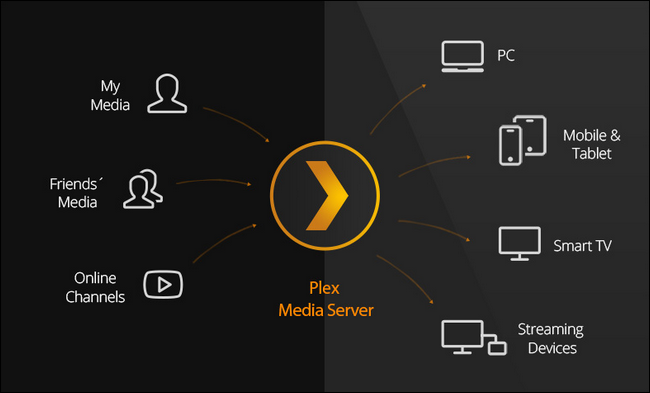
\includegraphics[width=.8\textwidth]{plex}
	\caption{Plex Platform}
	\label{fig:4.1}
\end{figure}
The Plex Media Server either running on Windows, macOS, Linux, FreeBSD or a NAS which organizes audio (music) and visual (photos and videos) content from personal media libraries and streams it to their player counterparts.
The players can either be the Plex Apps available for mobile devices, smart TVs, and streaming boxes, or the web UI of the Plex Media Server called Plex Web App, or the old Plex player called Plex Home Theater.\\
In particular Plex for Android application can connect to the media server to play its content and in addition it can search for Plex players in a LAN and send streamed content such as videos, movies or photo, to another player that can be also an Android device. In this way the Android Plex application client can behave like the Liquid Android system i want to develop. It can send a sort of \textit{Android intent}, to reproduce a media, from one device to another, and then it can send commands such as pause, rewind, forward and so on. The limits of such a system are that it is possible to send, and play, only multimedia contents, and only to devices which have the Plex app activity in foreground on the device.

\subsubsection{Goolgle Home and Cast API}
Google itself provides an application to control and send contents form an Android device, to some special devices in home network. \textit{Google Home} is an Android application which can find, setup, manage and control, Google's home devices like the \textit{Google Chromecast}. In this way is easy to setup and control and Android distributed system in which user can sent multimedia contents and command to the Google Home devices in the LAN. For these reason Google provides a development library, included in the Android framework, called \textit{Cast API} with which it is easy, for a developer, to build applications that can send multimedia streams to other Google devices specifically built for these purposes.\\
Also in this case the limitation is the kind of content, only multimedia, and also the type of devices involved which are limited number of special purposes devices.

\subsubsection{DroidMote and Remote control systems}
If we consider the possibility to control remote devices in a LAN, there are actually many different kind of applications that can do that also in an Android environment.
DroidMote is probably the most complete application to control remotely an Android device from another one. It is composed by two parts, the server, to be installed in the device to be controlled, and the client, to be installed in the one which controls. With this application is possible to control entirely the device running the server component: is it possible to open applications, perform tasks, open system settings and so on.\\
These kind of systems are capable to generate local intents in remote devices over a LAN but in a completely different way from I want to develop the solution to the given problem. In this case the \textit{controller} is explicitly controlling the remote device as it is using only the \textit{controlled} one. These systems are solution only to the problem of remote control, they can not exploit distributed Android devices computation power, in fact in an environment like this Android devices are not cooperating to perform task but one of them is only controlling another one.






%
% ------------------------------------------------------------------------ %6